% <!-- coding: utf-8 -->
\renewcommand{\monlhead}{Parcours}
\section{Parcours}
Un parcours dure 5 minutes, ce qui correspond à 333 mètres à 4 km/h.

Suivant le terrain et la densité d'oiseaux, cette longueur peut variée.

En cas de difficulté d'identification d'oiseaux (roitelet par exemple), la durée est augmentée.

Pour les points d'écoute, la longueur est nulle.

Les parcours sont enregistrés en format geojson. Les données sont ensuite traitées en R

\subsection{par observateur}
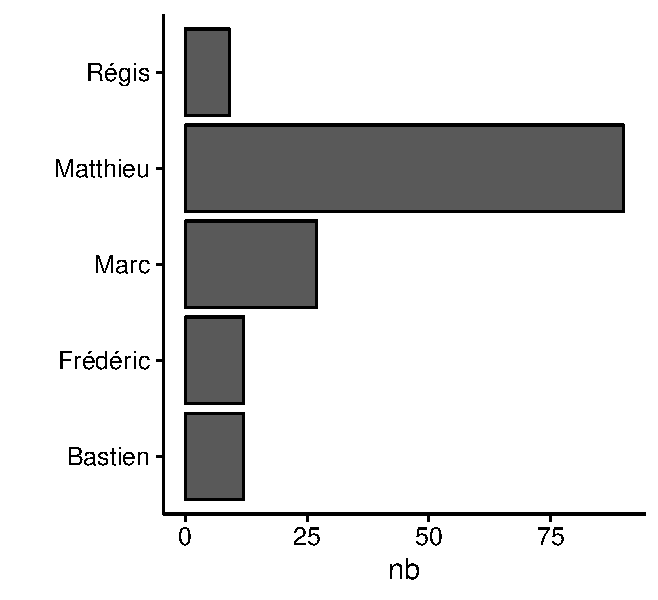
\includegraphics[width=\malargeurgraphique]{images/parcours_stat_champ_prenom.pdf}
\subsection{par longueur}
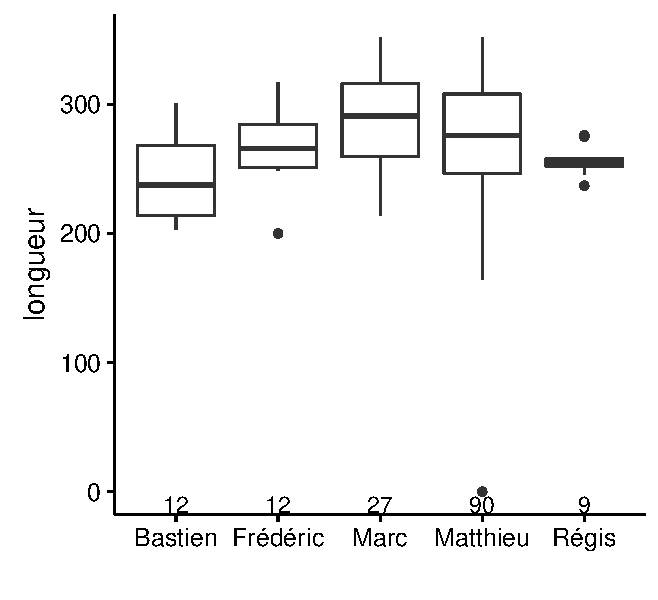
\includegraphics[width=\malargeurgraphique]{images/parcours_stat_email_longueur.pdf}
\subsection{carte}
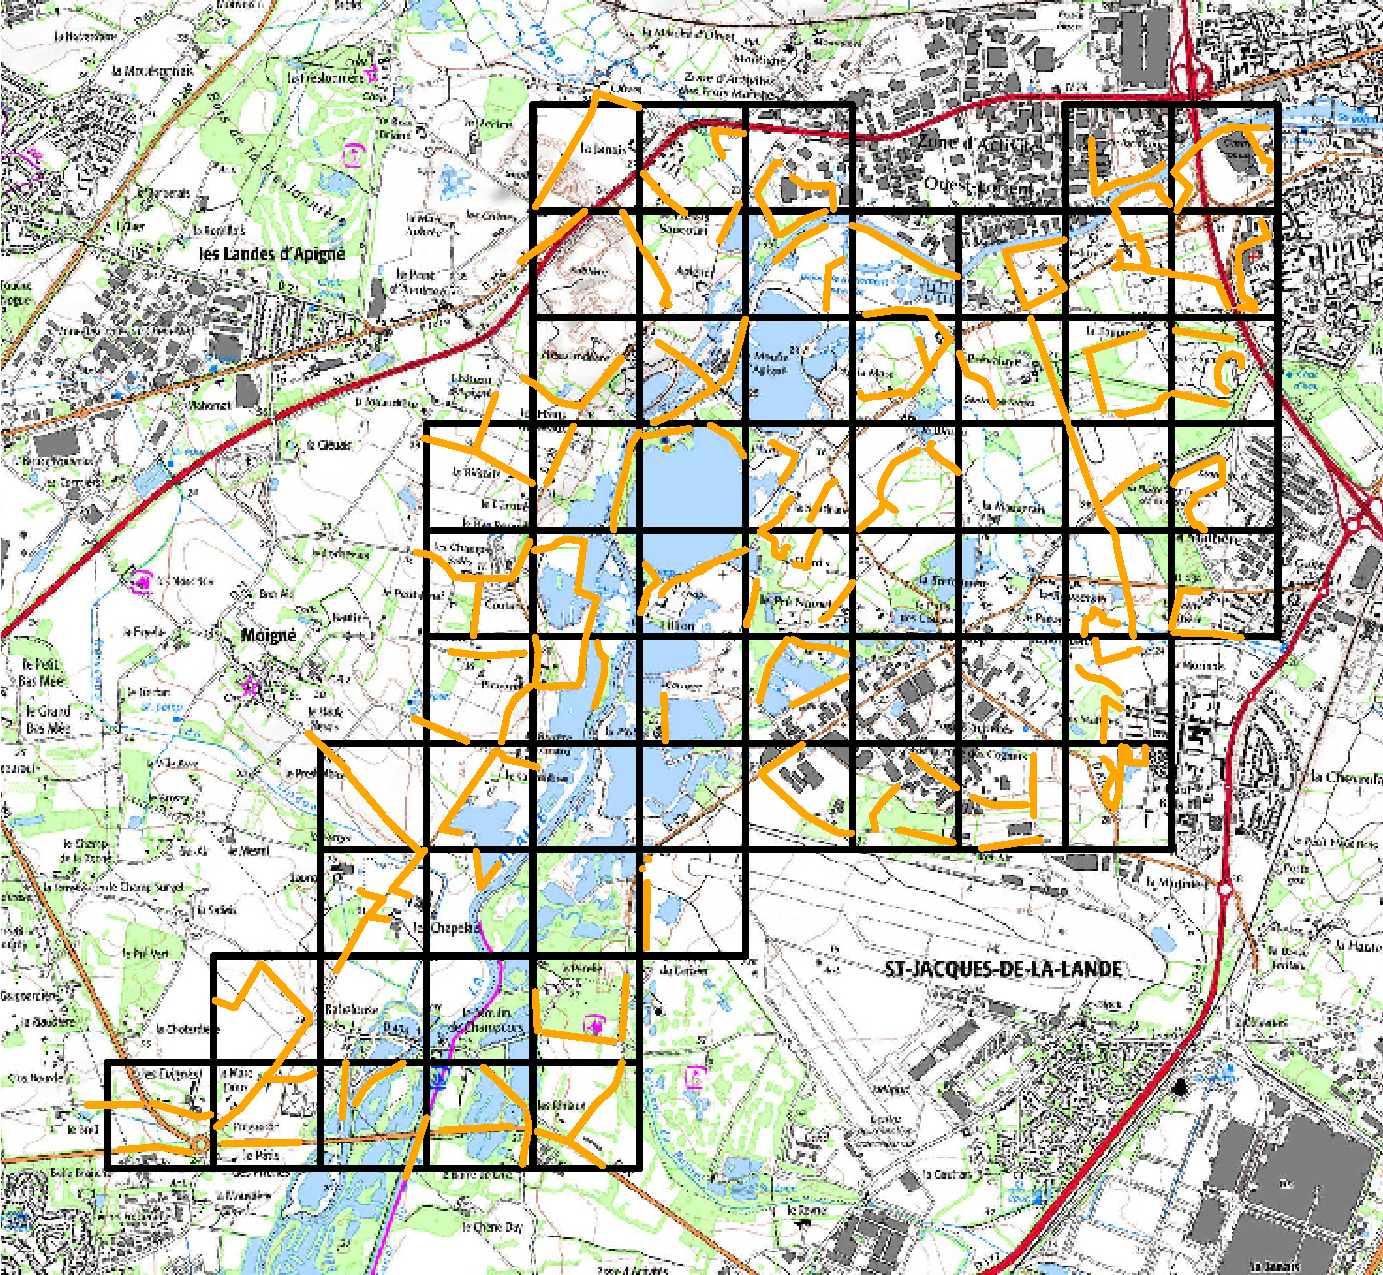
\includegraphics[width=\malargeurgraphique]{images/parcours_carte.pdf}
\clearpage
